\documentclass{beamer}

\usepackage[slovene]{babel}
\usepackage{amsfonts,amssymb}
\usepackage[utf8]{inputenc}
\usepackage{lmodern}
\usepackage[T1]{fontenc}

\usetheme{Warsaw}

\newtheorem{izrek}{Izrek}
\newtheorem{definicija}{Definicija}
\newtheorem{primer}{Primer}
\newtheorem{trditev}{Trditev}
\newtheorem{oznaka}{Oznaka}

\newcommand{\pojem}[1]{\textsc{#1}}


\title{Fareyevo zaporedje in Riemannova hipoteza}
\author{Tjaša Vrhovnik}

\institute{Mentor: izr.~prof.~dr.~Aleš Vavpetič\\
	Univerza v Ljubljani\\
	Fakulteta za matematiko in fiziko\\
	Oddelek za matematiko}
\date{10.\ december 2018}

\begin{document}

%%%%%%%%%%%%%%%%%%%%%%%%%%%%%%%%%%%%%%%%%%%

\begin{frame}
\titlepage
\end{frame}

%%%%%%%%%%%%%%%%%%%%%%%%%%%%%%%%%%%%%%%%%%%

\begin{frame}
\frametitle{Zgodovinski okvir}

\begin{itemize}
\item \emph{``The Ladies Diary: or, the Woman's Almanack''}, 1747
	Zanima nas število ulomkov različnih vrednosti, manjših od 1, katerih imenovalec ni večji od 100.
\item R. Flitcon, 1751: rešitev je 3003
\item Charles Haros
\item Henry Goodwyn
\item John Farey, 1816
\end{itemize}

\end{frame}

%%%%%%%%%%%%%%%%%%%%%%%%%%%%%%%%%%%%%%%%%%%

\begin{frame}
\frametitle{Fareyevo zaporedje}

\begin{definicija}
\pojem{Fareyevo zaporedje} reda n oz.\ n-to Fareyevo zaporedje je množica racionalnih števil $\frac{p}{q}$ urejenih po velikosti, kjer sta $p$ in $q$ tuji si števili, ter velja $0 \leq p \leq q \leq n$. Označimo ga z $F_n$.

Ekvivalentno, $F_n$ vsebuje vse okrajšane ulomke med 0 in 1 z imenovalci, kvečjemu enakimi $n$.
\end{definicija}

\pause
\begin{primer}
\(F_1 = \{\frac{0}{1}, \frac{1}{1}\} \)

\(F_2 = \{\frac{0}{1}, \frac{1}{2}, \frac{1}{1}\} \)

\(F_3 = \{\frac{0}{1}, \frac{1}{3}, \frac{1}{2}, \frac{2}{3}, \frac{1}{1}\} \)

\(F_4 = \{\frac{0}{1}, \frac{1}{4}, \frac{1}{3}, \frac{1}{2}, \frac{2}{3}, \frac{3}{4}, \frac{1}{1}\} \)

\(F_5 = \{\frac{0}{1}, \frac{1}{5}, \frac{1}{4}, \frac{1}{3}, \frac{2}{5}, \frac{1}{2}, \frac{3}{5}, \frac{2}{3}, \frac{3}{4}, \frac{4}{5}, \frac{1}{1}\} \)
\end{primer}

\end{frame}

%%%%%%%%%%%%%%%%%%%%%%%%%%%%%%%%%%%%%%%%%%%

\begin{frame}
\frametitle{Fareyevo zaporedje}

\begin{definicija}
Naj bosta $\frac{a}{b}$ in $\frac{c}{d}$ sosednja člena Fareyevega zaporedja. Člen \[\frac{a+c}{b+d} \] imenujemo \pojem{medianta}.
\end{definicija}

\pause
\begin{trditev}
Naj velja \( 0 \leq \frac{a}{b} < \frac{c}{d} \leq 1\). $\frac{a}{b}$ in $\frac{c}{d}$ sta Fareyeva soseda v $F_n$ natanko tedaj, ko velja \(bc - ad = 1\).
\end{trditev}

\end{frame}

%%%%%%%%%%%%%%%%%%%%%%%%%%%%%%%%%%%%%%%%%%%

\begin{frame}
\frametitle{Fareyevo zaporedje}

\begin{definicija}
Naj bo $\varphi(n)$ Eulerjeva funkcija. Dolžina Fareyevega zaporedja je
\[  |F_{n}| = |F_{n-1}| + \varphi(n). \]
\end{definicija}

\pause
\begin{trditev}
Asimptotično se dolžina Fareyevega zaporedja obnaša kot
\[  |F_{n}|\sim\frac{3n^2}{\pi^2}. \]
\end{trditev}

\end{frame}

%%%%%%%%%%%%%%%%%%%%%%%%%%%%%%%%%%%%%%%%%%%%

\begin{frame}
\frametitle{Fibonaccijevo zaporedje}

\begin{definicija}
Zaporedje Fibonaccijevih ulomkov definiramo kot
\[ \frac{1}{2}, \frac{1}{3}, \frac{2}{5}, \frac{3}{8}, \dots , \frac{\varphi_m}{\varphi_{m+2}}, \dots \]
\end{definicija}

\pause
\begin{trditev}
Sosednja Fibonaccijeva ulomka sta Fareyeva soseda.
\end{trditev}

\end{frame}

%%%%%%%%%%%%%%%%%%%%%%%%%%%%%%%%%%%%%%%%%%%

\begin{frame}
\frametitle{Fordovi krogi}

\begin{definicija}
\pojem{Fordov krog} C($\frac{p}{q}$) je krog v zgornji polravnini, ki se abscisne osi dotika v točki $\frac{p}{q}$ in ima polmer $\frac{1}{2q^2}$. Pri tem sta p in q tuji si števili. 
\end{definicija}

\begin{center}
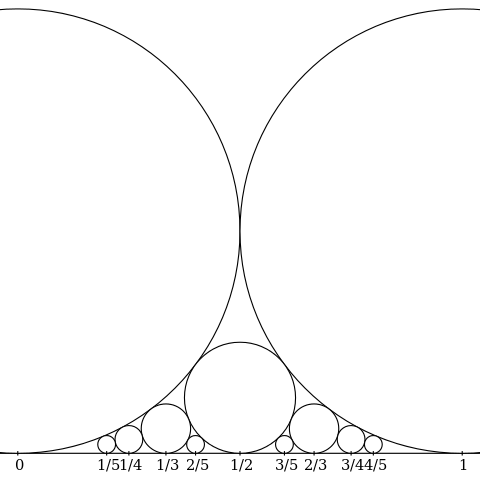
\includegraphics[scale=0.3]{fordov-krog.png}
\end{center}

\end{frame}

%%%%%%%%%%%%%%%%%%%%%%%%%%%%%%%%%%%%%%%%%%%

\begin{frame}
\frametitle{Riemannova hipoteza}

\begin{itemize}
\item Bernhard Riemann (1826 -- 1866)
\item obnašanje praštevil
\end{itemize}

\begin{center}
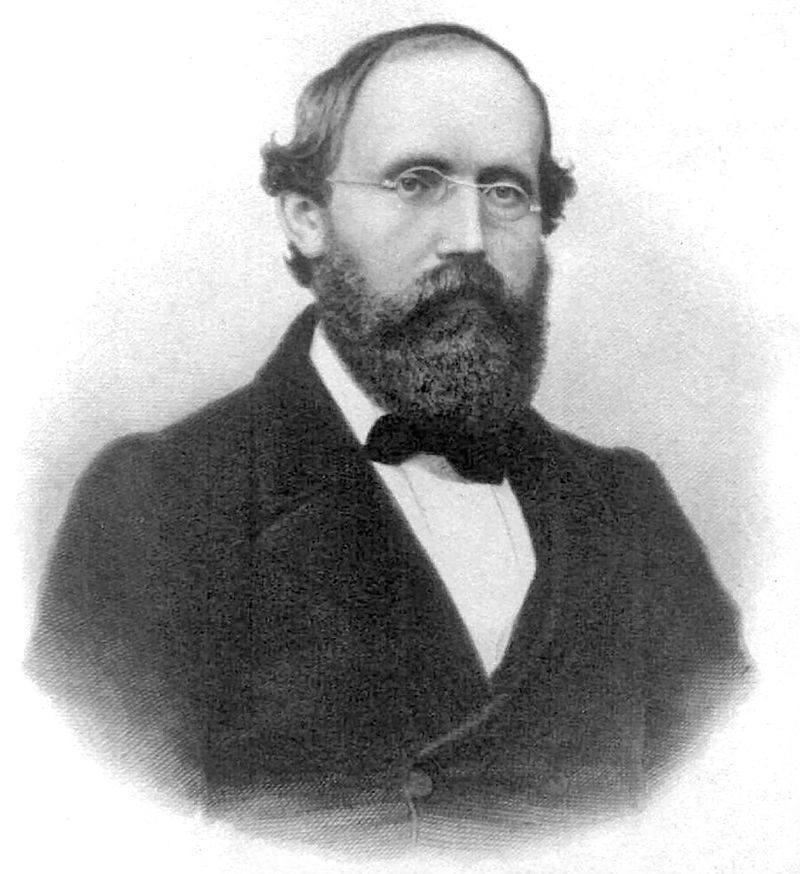
\includegraphics[scale=0.2]{riemann.png}
\end{center}

\end{frame}

%%%%%%%%%%%%%%%%%%%%%%%%%%%%%%%%%%%%%%%%%%%

\begin{frame}
\frametitle{Riemannova hipoteza}

\begin{definicija}
\pojem{Riemannova funkcija zeta} je za
 $s\in\mathbb{C}\backslash\{1\}$
definirana kot
\[ \zeta(s) = \sum_{n=1}^{\infty}\frac{1}{n^s}. \]
\end{definicija}

\[ \zeta(s) = \prod_{p}\frac{1}{1-p^{-s}}=\frac{1}{1-2^{-s}}\cdot\frac{1}{1-3^{-s}}\cdot\frac{1}{1-5^{-s}}\cdots \]

\pause
\begin{block}{Riemannova hipoteza}
Vse netrivialne ničle Riemannove funkcije zeta ležijo na premici $s=\frac{1}{2}+it$.
\end{block}

\end{frame}

%%%%%%%%%%%%%%%%%%%%%%%%%%%%%%%%%%%%%%%%%%%

\begin{frame}
\frametitle{Riemannova hipoteza}

\begin{definicija}
\pojem{M\"obiusova funkcija} je definirana kot
\[
\mu(k) = \left\{
\begin{array}{rl}
0 & ;\ \mbox{k vsebuje kvadrat}\\
(-1)^p & ;\  \mbox{k je produkt p različnih praštevil.}
\end{array}
\right.
\]
\end{definicija}

\begin{definicija}
\pojem{Mertensova funkcija} je definirana kot
\[ M(n)=\sum_{k\leq n}\mu(k).\]
\end{definicija}

\end{frame}

%%%%%%%%%%%%%%%%%%%%%%%%%%%%%%%%%%%%%%%%%%%

\begin{frame}
\frametitle{Riemannova hipoteza}

\begin{definicija}
Naj bosta $L(n)$ dolžina Fareyevega zaporedja $F_{n}$ in $r_{v}$ njegov v-ti element. Definiramo razliko
\[ \delta_{v}= r_{v}-v/L(n). \]
\end{definicija}

\begin{primer}
\[ F_5 = \{\frac{0}{1}, \frac{1}{5}, \frac{1}{4}, \frac{1}{3}, \frac{2}{5}, \frac{1}{2}, \frac{3}{5}, \frac{2}{3}, \frac{3}{4}, \frac{4}{5}, \frac{1}{1}\} \]
\[ L(5) = 11 \]
\[ \delta_{1} = \frac{0}{1} - \frac{1}{11} = -\frac{1}{11} \]
\[ \delta_{2} = \frac{1}{5} - \frac{2}{11} = \frac{1}{55} \]
\end{primer}

\end{frame}

%%%%%%%%%%%%%%%%%%%%%%%%%%%%%%%%%%%%%%%%%%%

\begin{frame}
\frametitle{Riemannova hipoteza}

Za vsak $\varepsilon > 0$ 
\[ \sum_{v=1}^{L(n)}|\delta_{v}| = o(n^{1/2+\varepsilon}) \iff M(n) = o(n^{1/2+\varepsilon}). \]

\end{frame}

%%%%%%%%%%%%%%%%%%%%%%%%%%%%%%%%%%%%%%%%%%%

\end{document}